\documentclass{article}
\usepackage{listings}
\usepackage{fullpage}
\usepackage{graphicx}
\usepackage{amsmath}
\usepackage{amsfonts}
\usepackage{amsthm}
\usepackage{subcaption}
\usepackage{mathtools}
\theoremstyle{definition}
\newtheorem{definition}{Definition}[section]
\begin{document}
\section{Maximum clique decision problem}
Given a graph $G=(V,E)$ and an integer $k$, find a subgraph of $G$ of size $k$ isomorphic to $K_k$. In this case we are only interested in getting a yes/no answer.
\section{Constraint programming}
A constraint modelling language MiniZinc was used to model the problem. Each model has variables and constraints. Each variable has a domain of possible values.

For each variable, a constraint solver keeps either its current value or a subset of its domain that it still deems possible. It then repeats the following two steps:
\begin{enumerate}
\item Inference. For each constraint and for each possible value in each (remaining) domain, check if that value is still possible.
\item Search. Choose a free variable according to a heuristic and choose one of its possible values according to some rule. Set the variable equal to that value and recurse.
\end{enumerate}
\section{Models}
\subsection{Initial}
\begin{lstlisting}
include "globals.mzn";

int: n; % number of vertices
int: k; % size of the clique we're looking for
array[1..n,1..n] of 0..1: adjacent; % adjacency matrix
array[1..n] of var 0..1: clique; % whether a vertex is part of the clique

constraint sum(clique) == k;
constraint forall(i, j in 1..n where i != j)(
    clique[i] == 1 /\ clique[j] == 1 -> adjacent[i,j] == 1);
solve satisfy;
\end{lstlisting}
A script was implemented to generate graphs with a set number of vertices and a probability of having an edge between every two vertices.
\begin{figure}
  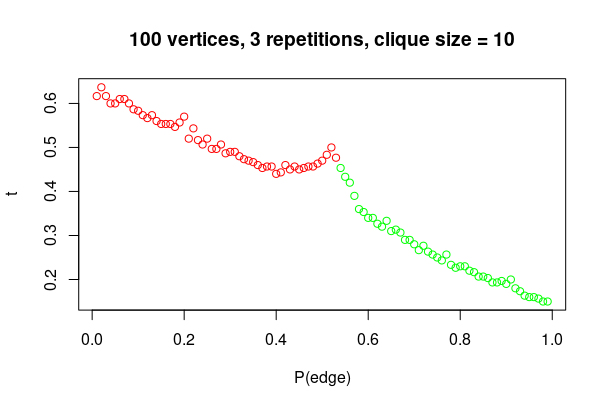
\includegraphics[scale=0.5]{max_clique.png}
  \caption{First model}
  \label{fig:initial_max_clique}
\end{figure}
Figure \ref{fig:initial_max_clique} shows how the running time (in seconds) changed by changing the edge probability for a graph with 100 vertices looking for a clique of size 10, averaged out over 3 different graphs. Each data point is marked green if a clique of required size was found most of the time (2 out of 3 runs) and red otherwise.

Surprisingly, this model takes the longest time for graphs with almost no edges. To explain that, consider two things: 1) how guesses are ordered during the search, and 2) when inference can actually reduce domain sizes.

Usually, variables are ordered by domain size, but in this case all domains are of size 2, so the actual ordering is essentially random. The algorithm has no way of knowing which values it should try first, so the default ordering is ascending, which means that we are guessing which vertices are not in the clique until all the remaining vertices have to be in the clique. Hence, switching the order could reduce the average height of the search tree. The variable ordering could also be improved by ordering vertices by their degree in either ascending or descending order.

The first constraint is easily checked and marks the remaining vertices as part of the clique once that is the only way to satisfy the constraint. According to the optimized FlatZinc file, the second constraint is actually transformed to its contrapositive and for every non-edge, it checks that one of the incident vertices is not in the clique. For sparse graphs, that is $O(|V|^2)$ of work.
\subsection{Small improvements}
To produce a more optimized FlatZinc file, the number of constraints was reduced in half by considering each pair of vertices only once (enforcing $j<i$). Taking the contrapositive of the main constraint allows the FlatZinc constraint to be expressed as an inequality instead of a logical OR.
\begin{lstlisting}
include "globals.mzn";

int: n; % number of vertices
int: k; % size of the clique we're looking for
array[1..n,1..n] of 0..1: adjacent; % adjacency matrix
array[1..n] of var 0..1: clique; % whether a vertex is part of the clique

constraint sum(clique) == k;
constraint forall(i in 1..n, j in 1..i-1 where adjacent[i,j] == 0)(
    clique[i] + clique[j] <= 1);
solve satisfy;
\end{lstlisting}
\begin{figure}
  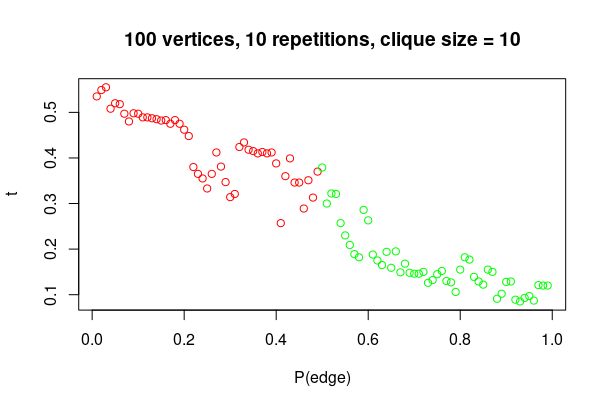
\includegraphics[scale=0.5]{max_clique2.png}
  \label{fig:second_max_clique}
  \caption{Second model}
\end{figure}
This model had more variance in its performance, especially around the transition from negative to positive answers. The number of repetitions was increased to 10. The general (downward) trend remains the same.
\subsection{Fixing value ordering}
A search annotation was added to try assigning vertices to the clique instead of assigning vertices to not be in the clique.
\begin{lstlisting}
include "globals.mzn";

int: n; % number of vertices
int: k; % size of the clique we're looking for
array[1..n,1..n] of 0..1: adjacent; % adjacency matrix
array[1..n] of var 0..1: clique; % whether a vertex is part of the clique

constraint sum(clique) == k;
constraint forall(i in 1..n, j in 1..i-1 where adjacent[i,j] == 0)(
    clique[i] + clique[j] <= 1);
solve :: int_search(clique, first_fail, indomain_max, complete)
    satisfy;
\end{lstlisting}
\begin{figure}
  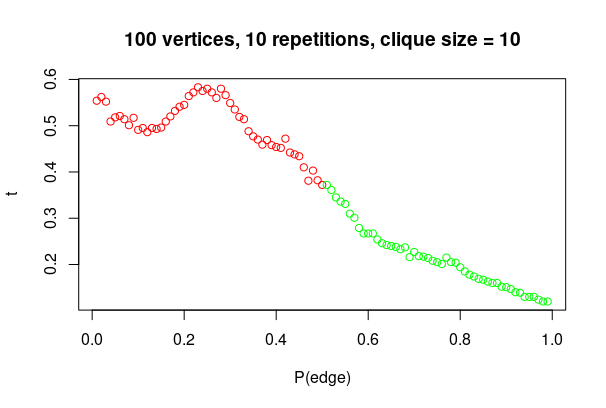
\includegraphics[scale=0.5]{max_clique3.png}
  \label{fig:third_max_clique}
  \caption{Third model}
\end{figure}
Several interesting changes happened to the running time plot:
\begin{enumerate}
\item The peak that used to mark the transition from negative to positive answers now shifted to the left.
\item Sparse graphs are still hard to deal with, but not as hard as average negative cases, with around 0.3 edge probability.
\end{enumerate}
\subsection{Variable ordering}
The variable choice annotation was changed to \texttt{input\_order} and the graph generator was updated to sort the vertices by their degree in a descending order so that the search algorithm considers putting the highest-degree vertices into the clique before others. That did not affect the results in any way. Reversing the sort order did nothing as well.
\section{Observations}
\begin{figure}
  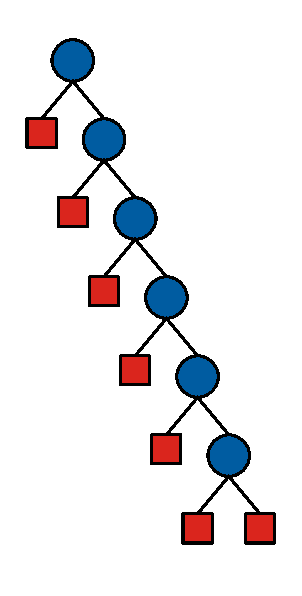
\includegraphics[scale=0.5]{search_tree.pdf}
  \label{fig:search_tree}
  \caption{The search tree for a graph with 10 vertices and no edges, looking for a clique of size 4}
\end{figure}
According to a visualization tool Gist, for a graph with no edges, the search tree is optimal: the algorithm is repeatedly picking each vertex to be in the clique and inferring that all the other vertices have to be outside it, which makes reaching a clique of size greater than 1 impossible. It continues to do so $|V|-k+1$ times, where $k$ is the size of the clique, because setting that last vertex to not be in the clique would make the clique size constraint impossible to satisfy. Therefore, the only other reason this model could be slow for sparse graphs is because sparse graphs have more constraints that need to be checked. The general equation for the number of constraints for this model is $\frac{n(n-1)}{2}-m+1$, for a graph with $n$ vertices and $m$ edges, which is bigger for sparse graphs.
\section{Subsequent attempts}
\subsection{Only consider vertices of high enough degree}
Every vertex that can possibly be in a clique of size $k$ must have a degree of at least $k-1$. Thus, instead of having $|V|$ variables, we can pre-filter which vertices fit this condition and only consider those.
\begin{lstlisting}
include "globals.mzn";

int: n; % number of vertices
int: k; % size of the clique we're looking for
array[1..n,1..n] of 0..1: adjacent; % adjacency matrix
% a vertex i can be part of a clique of size k only if deg(i) >= k - 1
set of 1..n: possible = {i | i in 1..n where sum(j in 1..n)(
    adjacent[i,j]) >= k - 1};
array[possible] of var 0..1: clique; % whether a vertex is part of the clique

constraint sum(clique) == k;
constraint forall(i, j in possible where i < j)(
    adjacent[i,j] == 0 -> clique[i] + clique[j] <= 1);
solve :: int_search(clique, input_order, indomain_max, complete)
    satisfy;
\end{lstlisting}
\begin{figure}
  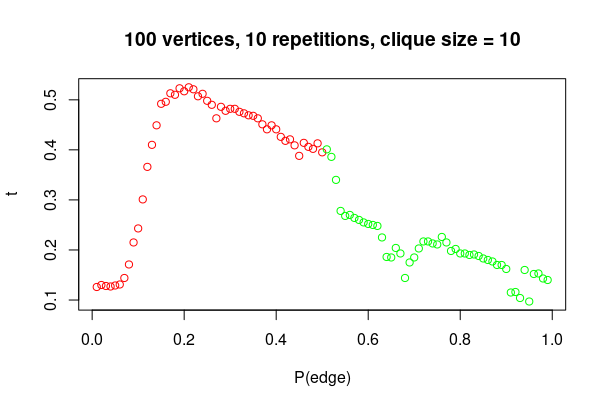
\includegraphics[scale=0.5]{max_clique4.png}
  \caption{Fourth model}
  \label{fig:fourth_max_clique}
\end{figure}
According to Figure \ref{fig:fourth_max_clique}, this reduces the running time for graphs with $P(\text{edge}) < 0.1$, however slightly denser sparse graphs remain hard to solve.
\subsection{Modifying model running script}
Model running script was modified to track all the available statistical information as well as running time. At this point it became easier to take the running time information from the statistics rather than running an external command \texttt{time}. The new running time is 0 for almost all graphs with the answer NO. The script was modified again to run \texttt{mzn2fzn} followed by \texttt{fzn-gecode} instead of \texttt{mzn-gecode}. That makes the NO instances have more realistic running time properties.
\begin{figure}
  \begin{subfigure}{.5\textwidth}
    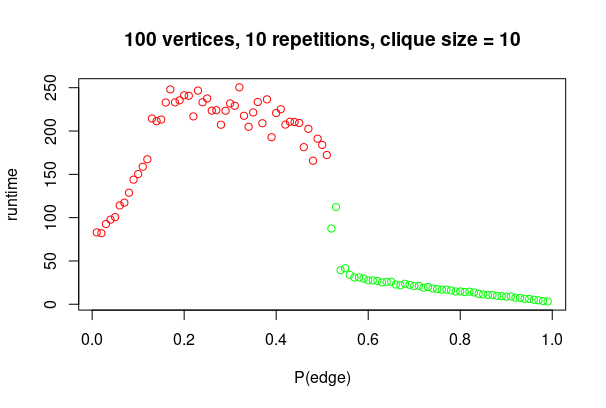
\includegraphics[scale=0.5]{3_runtime.png}
    \caption{Running time}
    \label{fig:3_runtime}
  \end{subfigure}
  \begin{subfigure}{.5\textwidth}
    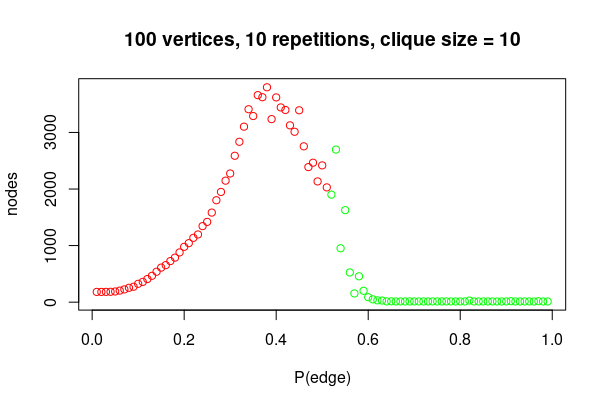
\includegraphics[scale=0.5]{3_nodes.png}
    \caption{Number of nodes in the search tree}
    \label{fig:3_nodes}
  \end{subfigure}
  \caption{Properties of the third model with the new measuring system}
  \label{fig:3_properties}
\end{figure}
\begin{figure}
  \begin{subfigure}{.5\textwidth}
    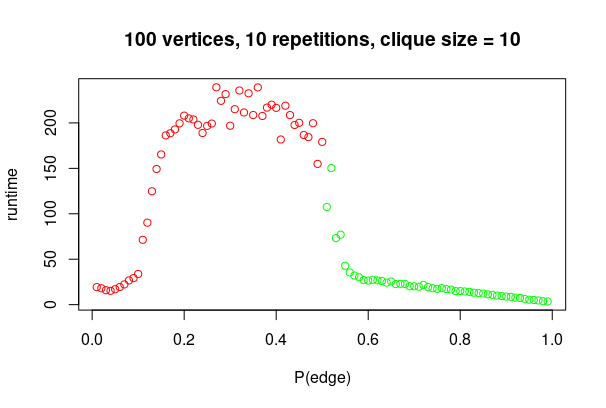
\includegraphics[scale=0.5]{4_runtime.png}
    \caption{Running time}
    \label{fig:4_runtime}
  \end{subfigure}
  \begin{subfigure}{.5\textwidth}
    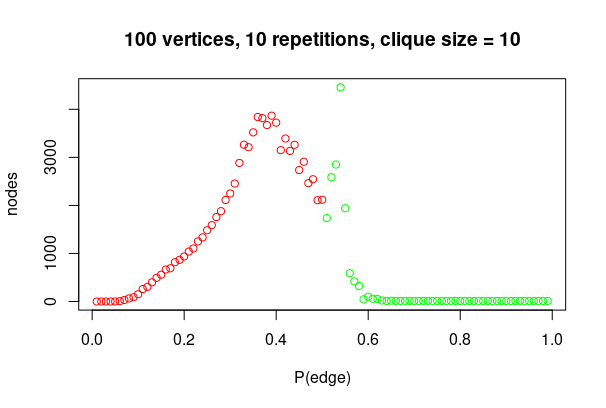
\includegraphics[scale=0.5]{4_nodes.png}
    \caption{Number of nodes in the search tree}
    \label{fig:4_nodes}
  \end{subfigure}
  \caption{Properties of the fourth model with the new measuring system}
  \label{fig:4_properties}
\end{figure}
Figures \ref{fig:3_properties} and \ref{fig:4_properties} show properties of the third and fourth models measured in this new way, tracking both running time and number of nodes in the search tree. The one suspicious observation is how dense graphs have basically no search tree nodes. However, according to the dataset, the number of search tree nodes for dense graphs is around 11-12, which sounds reasonable when looking for a clique of size 10.
\subsection{Mathematical modelling}
The distribution of the number of search tree nodes looks reasonable. We have an exact equation for the number of constraints for model 3 (we choose model 3 because it is more predictable and the additional optimization introduced in model 4 only affects very sparse graphs). We are going to prove that running time can be approximated as nodes $\times$ constraints. The number of constraints is $\frac{n(n-1)}{2}-m+1$. For a graph with edge probability $p$, $\mathbb{E}[m] = \frac{n(n-1)p}{2}$. So the expected number of constraints is
\[ \frac{n(n-1)}{2}-\frac{n(n-1)p}{2}+1=\frac{n(n-1)(1-p)}{2}+1. \]
Thus, we claim that running time can be approximated by
\[ \text{nodes}\times \left( \frac{n(n-1)(1-p)}{2} + 1 \right). \]
Since all our experiments were with 100-vertice graphs, substituting $n=100$ gives
\begin{equation}
  \text{nodes} \times (4950(1-p)+1).
  \label{eq:model}
\end{equation}
Using the existing data for the number of nodes and $p$ gives the graph in Figure \ref{fig:model}, which compares the actual running time with the one given in equation \ref{eq:model}, scaled so that the mean values would be equal.
\begin{figure}
  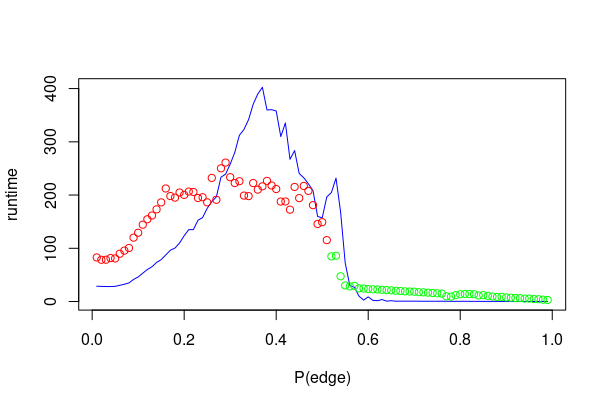
\includegraphics[scale=0.5]{model.png}
  \caption{Real running time compared with the estimate (blue)}
  \label{fig:model}
\end{figure}
Our mathematical model is overestimating average cases and underestimating sparse cases, which could be explained by additional setup time required by the algorithm. Running a linear regression
\[ \mathbb{E}[\text{runtime}] = \alpha * \text{prediction} + \beta \]
gives Figure \ref{fig:regression}, p-value of $ < 2.2\times 10^{-16}$, and adjusted $R^2 = 69.36\%$.

Now that we know such a powerful predictor of running time, we can examine its components in more detail. The number of nodes in the search tree is basically what we would expect and we already examined the search tree for sparse graphs to see that it is not doing anything particularly inefficient. The number of constraints is more interesting. We explored the basic definition of what a clique is in both directions (from two vertices being in a clique and from two vertices not sharing an edge). When MiniZinc code is optimized to FlatZinc, the direction of going from a premise without variables to a conclusion with variables is always preferred. This means that without having an alternative definition of a clique, the running time plot cannot be changed in a significant way (other than reducing the running time for all cases without changing its plot or optimizations such as our model 4).
\begin{figure}
  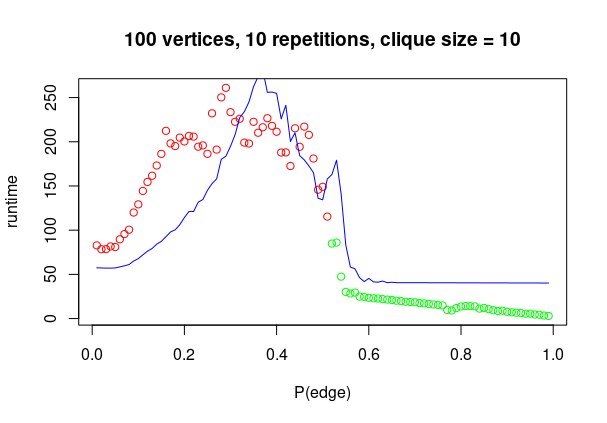
\includegraphics[scale=0.5]{regression.png}
  \caption{The resulting curve of the linear regression compared with the real data}
  \label{fig:regression}
\end{figure}
\subsection{Multiple linear regression}
To see how good our running time estimate can get, we ran multiple linear regression by adding the number of constraints and the number of nodes as explanatory variables. The resulting model, plotted in Figure \ref{fig:regression2}, has $R^2 = 89.36\%$ and every parameter (except the intercept) is highly significant.
\begin{figure}
  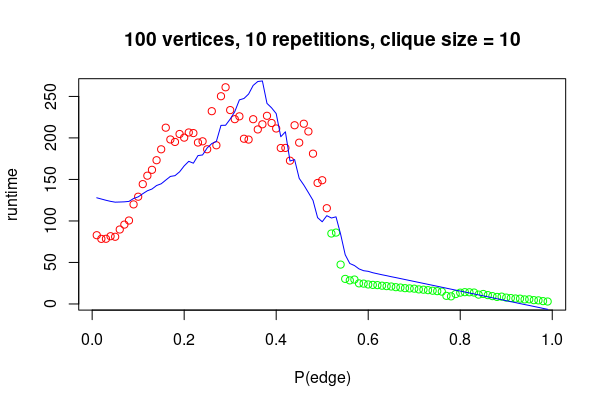
\includegraphics[scale=0.5]{regression2.png}
  \caption{Multiple linear regression}
  \label{fig:regression2}
\end{figure}
\section{Induced subgraph isomorphism}
Let $G = (V, E)$, $H = (V', E')$ be graphs. Does there exist an injective function $f: V' \to V$ such that $(v_1, v_2) \in E' \iff (f(v_1), f(v_2)) \in E$?
\subsection{First CP model}
\begin{lstlisting}
include "globals.mzn";

% checking if graph 2 is isomorphic to a subgraph of graph 1
int: n1;
int: n2;
array[1..n1,1..n1] of 0..1: adjacent1;
array[1..n2,1..n2] of 0..1: adjacent2;
% a function from vertices of graph 2 to vertices of graph 1
array[1..n2] of var 1..n1: isomorphism;

constraint all_different(isomorphism); % injectivity
constraint forall(i in 1..n2, j in 1..i-1)(
    adjacent2[i,j] == 1 <-> adjacent1[isomorphism[i], isomorphism[j]] == 1);
solve satisfy;
\end{lstlisting}
The pattern had 8 vertices and a constant edge probability of 0.5. The target had 40 vertices and a varying edge probability from 0.01 to 1 in steps of 0.01. Each point on the plot corresponds to an average of 3 runs with both graphs being regenerated each time. The results are in Figure \ref{fig:subgraph_properties} and they are not surprising.
\begin{figure}
  \begin{subfigure}{.5\textwidth}
    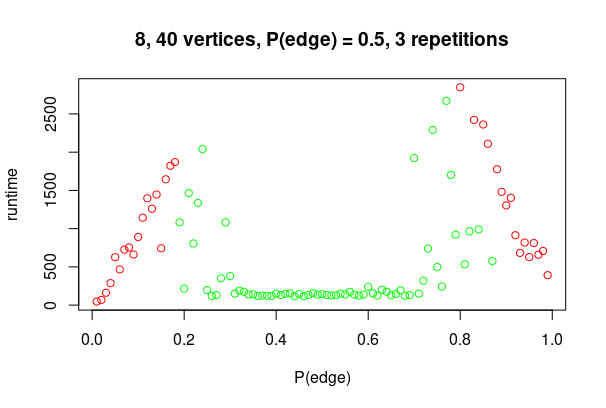
\includegraphics[scale=0.5]{subgraph_runtime.png}
    \caption{Running time}
  \end{subfigure}
  \begin{subfigure}{.5\textwidth}
    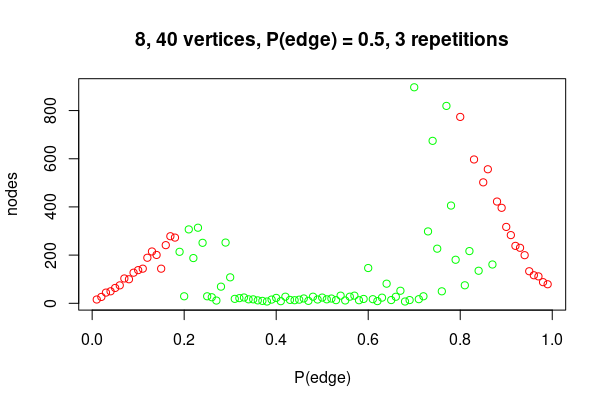
\includegraphics[scale=0.5]{subgraph_nodes.png}
    \caption{Number of nodes in the search tree}
  \end{subfigure}
  \caption{Properties of the first model for the subgraph isomorphism problem}
  \label{fig:subgraph_properties}
\end{figure}
\section{Maximum common induced subgraph}
Let $G_1 = (V_1, E_1), G_2 = (V_2, E_2) $ be graphs, where $ V_1 = \{v_{1,i}: 1 \le i \le n\}$, $ V_2 = \{v_{2,i}: 1 \le i \le m\}$. For maximum common induced subgraph (MCIS) problem, we are looking for a third graph that is an induced subgraph of both $G_1$ and $G_2$. The MiniZinc model is as follows:
\begin{lstlisting}
include "globals.mzn";

int: n1;
int: n2;
array[1..n1,1..n1] of 0..1: adjacent1;
array[1..n2,1..n2] of 0..1: adjacent2;
% a function from vertices of graph 2 to vertices of graph 1; 0 means not mapped
array[1..n2] of var 0..n1: isomorphism;
var 0..min(n1, n2): size;

constraint size == sum([1 | i in isomorphism where i != 0]);
constraint alldifferent_except_0(isomorphism);
constraint forall(i in 1..n2, j in 1..i-1
    where isomorphism[i] != 0 /\ isomorphism[j] != 0)(
    adjacent2[i,j] == 1 <-> adjacent1[isomorphism[i], isomorphism[j]] == 1);
solve maximize size;

output [show(size)];
\end{lstlisting}
\subsection{Reduction to max clique}
Create a new graph $G_3 = (V_3, E_3)$, where $V_3 = \{u_{i,j}: 1 \le i \le n, 1 \le j \le m\}$ and $E_3 = \{\{u_{i,j}u_{k,l}\}: i \ne k, j \ne l, (\{v_{1,i}v_{1,k}\} \in E_1 \iff \{v_{2,j}v_{2,l}\} \in E_2)\}$. Max clique on $G_3$ corresponds to MCIS between $G_1$ and $G_2$. 
\begin{figure}
  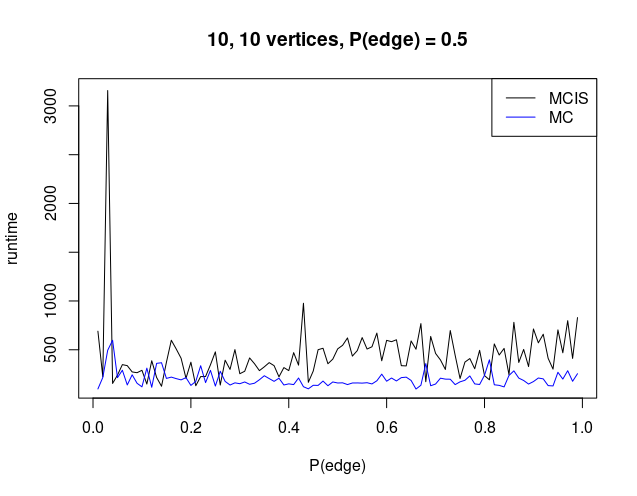
\includegraphics[scale=0.5]{conversion.png}
  \caption{Running times of the same problems solved with MCIS and MC}
  \label{fig:conversion}
\end{figure}
Figure \ref{fig:conversion} shows how the running times distributed for the two algorithms. Keep in mind that conversion time is not factored in here. Overall, MC is almost always faster and seems to have lower variance.
\subsection{Labelled vertices}
Each graph now has a probability for each vertex to have a label. Labels are assigned uniformly from $[1, |V_1| + |V_2|]$ so that all vertices could have different labels. The new MCIS model is as follows:
\begin{lstlisting}
include "globals.mzn";

int: n1;
int: n2;
array[1..n1,1..n1] of 0..1: adjacent1;
array[1..n2,1..n2] of 0..1: adjacent2;

% 0 means unlabelled
array[1..n1] of 0..n1+n2: vLabel1;
array[1..n2] of 0..n1+n2: vLabel2;

% a function from vertices of graph 2 to vertices of graph 1; 0 means not mapped
array[1..n2] of var 0..n1: isomorphism;
var 0..min(n1, n2): size;

constraint size == sum([1 | i in isomorphism where i != 0]); % defining size
constraint alldifferent_except_0(isomorphism); % injectivity
constraint forall(i in 1..n2, j in 1..i-1 % main constraint
    where isomorphism[i] != 0 /\ isomorphism[j] != 0)(
    adjacent2[i,j] == 1 <-> adjacent1[isomorphism[i], isomorphism[j]] == 1);
    
% preserving labels
constraint forall(j in 1..n2)(vLabel2[j] > 0 /\ isomorphism[j] != 0 ->
    vLabel1[isomorphism[j]] == vLabel2[j]);
constraint forall(i in 1..n1, j in 1..n2)(
    vLabel1[i] > 0 /\ isomorphism[j] == i -> vLabel2[j] == vLabel1[i]);

solve maximize size;
output [show(size)];
\end{lstlisting}
The new constraint says that an unlabelled vertex can only match other unlabelled vertices and a labelled vertex can only match another vertex with the same label. To encode this problem as MC, a vertex in $G_3$ is only created if the two vertices have the same label or both have no labels. If this happens to create an empty graph, the running time is recorded as 0. To compare MCIS and MC performance for vertex-labelled graphs, edge probability was kept constant for both graphs (as it seems to not be an interesting parameter for this problem), and only label probability was varied between runs. Results in Figure \ref{fig:conversion2} still show MC to be superior if we disregard the transformation time.
\begin{figure}
  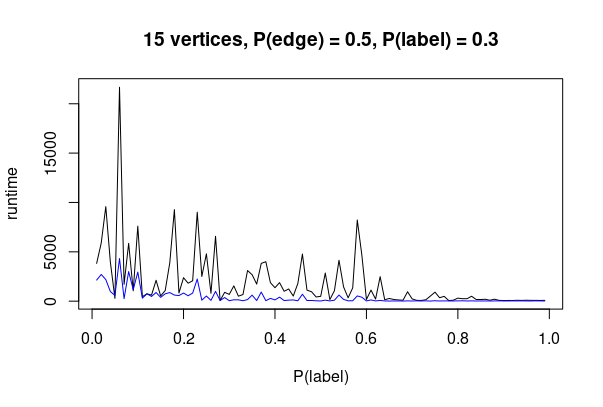
\includegraphics[scale=0.5]{conversion2.png}
  \caption{Comparing MCIS and MC for vertex-labelled graphs}
  \label{fig:conversion2}
\end{figure}
\section{Graph Edit Distance}
\begin{definition}
  An \emph{attributed graph} $G = (V, E, L_V, L_E, \mu, \zeta)$ is a 6-tuple where:
  \begin{itemize}
  \item $V$ is a set of vertices
  \item $E \subseteq V \times V$ is a set of edges
  \item $L_V$ is a set of vertex attributes
  \item $L_E$ is a set of edge attributes
  \item $\mu : V \to L_V$ is a vertex labellling function
  \item $\zeta : E \to L_E$ is an edge labelling function
  \end{itemize}
\end{definition}
\begin{definition}
  A function $f: V_1 \cup \{ \epsilon \} \to V_2 \cup \{ \epsilon \}$ is an \emph{error-tolerant GM} from $G_1 = (V_1, E_1, L_{V_1}, L_{E_1}, \mu_1, \zeta_1)$ to $G_2 = (V_2, E_2, L_{V_2}, L_{E_2}, \mu_2, \zeta_2)$ where $\epsilon$ refers to the empty vertex if
  \begin{enumerate}
  \item considering only non-empty vertices, $f: V_1 \to V_2$ is bijective,
  \item $\forall u_1, u_2 \in V_1, f(u_1) \ne \epsilon \implies f(u_1) \ne f(u_2)$,
  \item $\forall v_1, v_2 \in V_2, f^{-1}(v_1) \ne \epsilon \implies f^{-1}(v_1) \ne f^{-1}(v_2)$.
  \end{enumerate}
\end{definition}
\begin{definition}
  Let $f: V_1 \to V_2$ be an error-tolerant GM between graphs $G_1 = (V_1, E_1)$ and $G_2 = (V_2, E_2)$ and let $c: (V_1 \cup \{ \epsilon \} \times V_2 \cup \{ \epsilon \}) \cup (E_1 \cup \{ \epsilon \} \times E_2 \cup \{ \epsilon \}) \to \mathbb{R}$ be an arbitrary cost function. The \emph{matching cost function} of $f$ is defined as
  \[
  \begin{aligned}
    c(f) &= \overbrace{\sum_{\substack{u_i \in V_1\\ f(u_i) \in V_2}} c(u_i, f(u_i))}^{\mathclap{\text{vertex substitutions}}} + \overbrace{\sum_{\substack{u_i \in V_1\\ f(u_i) = \epsilon}} c(u_i, \epsilon)}^{\mathclap{\text{vertex deletions}}} + \overbrace{\sum_{\substack{v_k \in V_2\\ f^{-1}(v_k) = \epsilon}} c(\epsilon, v_k)}^{\mathclap{\text{vertex insertions}}} \\
    &+ \overbrace{\sum_{\substack{e(u_i, u_j) \in E_1\\ e(f(u_i), f(u_j)) \in E_2}} c(e(u_i, u_j), e(f(u_i), f(u_j)))}^{\mathclap{\text{edge substitutions}}} + \overbrace{\sum_{\substack{e(u_i, u_j) \in E_1\\ e(f(u_i), f(u_j)) = \epsilon}} c(e(u_i, u_j), \epsilon)}^{\mathclap{\text{edge deletions}}} \\
    &+ \overbrace{\sum_{\substack{e(v_k, v_l) \in E_2\\ e(f^{-1}(v_k), f^{-1}(v_l)) = \epsilon}} c(\epsilon, e(v_k, v_l))}^{\mathclap{\text{edge insertions}}}.
  \end{aligned}
  \]
\end{definition}
\begin{definition}
  A \emph{graph edit operation} for an attributed graph $G = (V, E, L_V, L_E, \mu, \zeta)$ is one of the following:
  \begin{itemize}
  \item vertex insertion ($V = V \cup \{ u_i \}$ for $u_i \not \in V$),
  \item vertex deletion ($V = V \setminus \{ u_i \}$ for $u_i \in V$),
  \item vertex substitution (redefine $\mu$ so that $\mu(u_i) = l_i$),
  \item edge insertion ($E = E \cup \{ e(u_i, u_j) \}$ for $e(u_i, u_j) \not \in E$, $u_i, u_j \in V$),
  \item edge deletion ($E = E \setminus \{ e(u_i, u_j) \}$ for $e(u_i, u_j) \in E$).
  \end{itemize}
\end{definition}
\begin{definition}
  A set $\{ ed_1, \dots, ed_k \}$ of $k$ edit operations $ed_i$ that transform a graph $G_1$ completely into another graph $G_2$ is called a (complete) \emph{edit path} $\lambda(G_1, G_2)$ between $G_1$ and $G_2$. A partial edit path refers to a subset of $\{ ed_1, \dots, ed_k \}$. The set of all complete edit paths is denoted $\gamma(G_1, G_2)$.
\end{definition}
\begin{definition}
  Let $G_1 = (V_1, E_1, L_{V_1}, L_{E_1}, \mu_1, \zeta_1)$ and $G_2 = (V_2, E_2, L_{V_2}, L_{E_2}, \mu_2, \zeta_2)$ be two attributed graphs and let $c$ be the cost function. The \emph{graph edit distance} between $G_1$ and $G_2$ is defined as
  \[ d_{\lambda_{\text{min}}}(G_1, G_2) = \min_{\lambda \in \gamma(G_1, G_2)} \sum_{ed_i \in \lambda} c(ed_i).\]
\end{definition}
\subsection{Implementation specifics}
To simplify encoding this problem as a CP model, we enforce that every vertex and every edge of both graphs must be part of some edit operation. Instead of not performing an edit operation, we can always do a substitution of cost 0.
\end{document}
